\documentclass{article}
% Change "article" to "report" to get rid of page number on title page
\usepackage{amsmath,amsfonts,amsthm,amssymb}
\usepackage{setspace}
\usepackage{Tabbing}
\usepackage{fancyhdr}
\usepackage{lastpage}
\usepackage{extramarks}
\usepackage{chngpage}
\usepackage{soul,color}
\usepackage{graphicx,float,wrapfig}
\usepackage{multirow}
\usepackage{enumerate}
% In case you need to adjust margins:
\topmargin=-0.45in      %
\evensidemargin=0in     %
\oddsidemargin=0in      %
\textwidth=6.5in        %
\textheight=9.0in       %
\headsep=0.25in         %

% Homework Specific Information
\newcommand{\hmwkTitle}{HDP:Dirichlet-Multinomial}
\newcommand{\hmwkClass}{}
\newcommand{\hmwkAuthorName}{Donglai\ Wei}


% Setup the header and footer
\pagestyle{fancy}                                                       %
\lhead{\hmwkAuthorName}                                                 %
\rhead{\firstxmark}                                                     %
\lfoot{\lastxmark}                                                      %
\cfoot{}                                                                %
\rfoot{Page\ \thepage\ of\ \pageref{LastPage}}                          %
\renewcommand\headrulewidth{0.4pt}                                      %
\renewcommand\footrulewidth{0.4pt}                                      %

% This is used to trace down (pin point) problems
% in latexing a document:
%\tracingall

%%%%%%%%%%%%%%%%%%%%%%%%%%%%%%%%%%%%%%%%%%%%%%%%%%%%%%%%\begin{enumerate}

% Some tools
\newcommand{\enterProblemHeader}[1]{\nobreak\extramarks{#1}{#1 continued on next page\ldots}\nobreak%
                                    \nobreak\extramarks{#1 (continued)}{#1 continued on next page\ldots}\nobreak}%
\newcommand{\exitProblemHeader}[1]{\nobreak\extramarks{#1 (continued)}{#1 continued on next page\ldots}\nobreak%
                                   \nobreak\extramarks{#1}{}\nobreak}%

\newlength{\labelLength}
\newcommand{\labelAnswer}[2]
  {\settowidth{\labelLength}{#1}%
   \addtolength{\labelLength}{0.25in}%
   \changetext{}{-\labelLength}{}{}{}%
   \noindent\fbox{\begin{minipage}[c]{\columnwidth}#2\end{minipage}}%
   \marginpar{\fbox{#1}}%

   % We put the blank space above in order to make sure this
   % \marginpar gets correctly placed.
   \changetext{}{+\labelLength}{}{}{}}%

\setcounter{secnumdepth}{0}
\newcommand{\homeworkProblemName}{}%
\newcounter{homeworkProblemCounter}%
\newenvironment{homeworkProblem}[1][Problem \arabic{homeworkProblemCounter}]%
  {\stepcounter{homeworkProblemCounter}%
   \renewcommand{\homeworkProblemName}{#1}%
   \section{\homeworkProblemName}%
   \enterProblemHeader{\homeworkProblemName}}%
  {\exitProblemHeader{\homeworkProblemName}}%

\newcommand{\problemAnswer}[1]
  {\noindent\fbox{\begin{minipage}[c]{\columnwidth}#1\end{minipage}}}%

\newcommand{\problemLAnswer}[1]
  {\labelAnswer{\homeworkProblemName}{#1}}

\newcommand{\homeworkSectionName}{}%
\newlength{\homeworkSectionLabelLength}{}%
\newenvironment{homeworkSection}[1]%
  {% We put this space here to make sure we're not connected to the above.
   % Otherwise the changetext can do funny things to the other margin

   \renewcommand{\homeworkSectionName}{#1}%
   \settowidth{\homeworkSectionLabelLength}{\homeworkSectionName}%
   \addtolength{\homeworkSectionLabelLength}{0.25in}%
   \changetext{}{-\homeworkSectionLabelLength}{}{}{}%
   \subsection{\homeworkSectionName}%
   \enterProblemHeader{\homeworkProblemName\ [\homeworkSectionName]}}%
  {\enterProblemHeader{\homeworkProblemName}%

   % We put the blank space above in order to make sure this margin
   % change doesn't happen too soon (otherwise \sectionAnswer's can
   % get ugly about their \marginpar placement.
   \changetext{}{+\homeworkSectionLabelLength}{}{}{}}%

\newcommand{\sectionAnswer}[1]
  {% We put this space here to make sure we're disconnected from the previous
   % passage

   \noindent\fbox{\begin{minipage}[c]{\columnwidth}#1\end{minipage}}%
   \enterProblemHeader{\homeworkProblemName}\exitProblemHeader{\homeworkProblemName}%
   \marginpar{\fbox{\homeworkSectionName}}%

   % We put the blank space above in order to make sure this
   % \marginpar gets correctly placed.
   }%

%%%%%%%%%%%%%%%%%%%%%%%%%%%%%%%%%%%%%%%%%%%%%%%%%%%%%%%%%%%%%



%%%%%%%%%%%%%%%%%%%%%%%%%%%%%%%%%%%%%%%%%%%%%%%%%%%%%%%%%%%%%
% Make title
\title{\vspace{0.3in}\textmd{\textbf{\hmwkTitle}}}
\date{2010.5.12}
\author{\textbf{\hmwkAuthorName}}
%%%%%%%%%%%%%%%%%%%%%%%%%%%%%%%%%%%%%%%%%%%%%%%%%%%%%%%%%%%%%

\begin{document}
\begin{spacing}{1.1}
\maketitle

\section{0)Problem}
Though ME algorithm can find an "almost good" log probability, the clustering result is far from truth. \\
The hope may lie in the "communicating power" among the dishes during {\bf Initialization} and {\bf Searching Tricks}.

Hyperparameters:$\alpha=0.5,\gamma=1.5,\phi_{0}=0.2$\\
\begin{figure}[h] 
  \begin{minipage}[b]{0.5\textwidth} 
    \centering 
    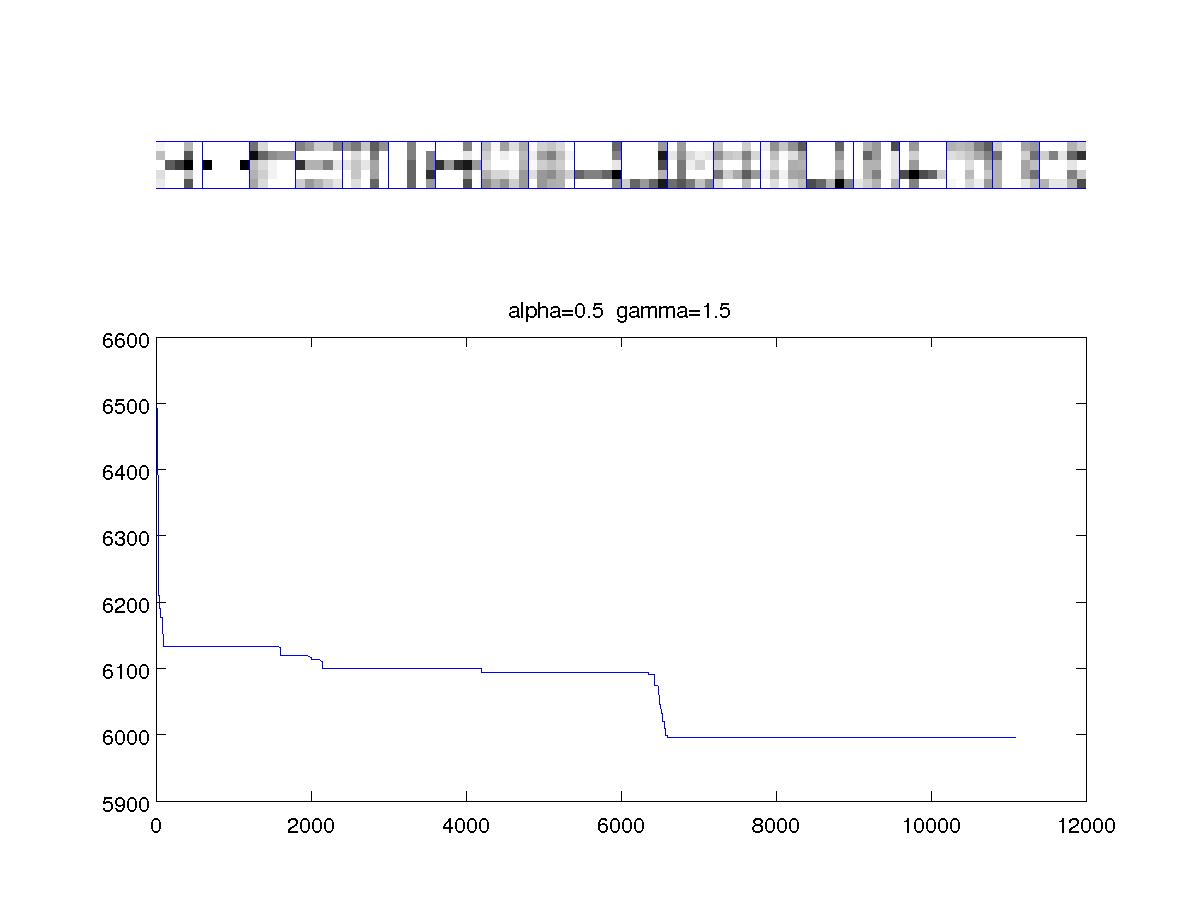
\includegraphics[width=3 in,height=2in]{exp_me1.jpg} 
    \caption{ME result} 
    \label{fig:by:table} 
  \end{minipage}% 
  \begin{minipage}[b]{0.5\textwidth} 
    \centering 
    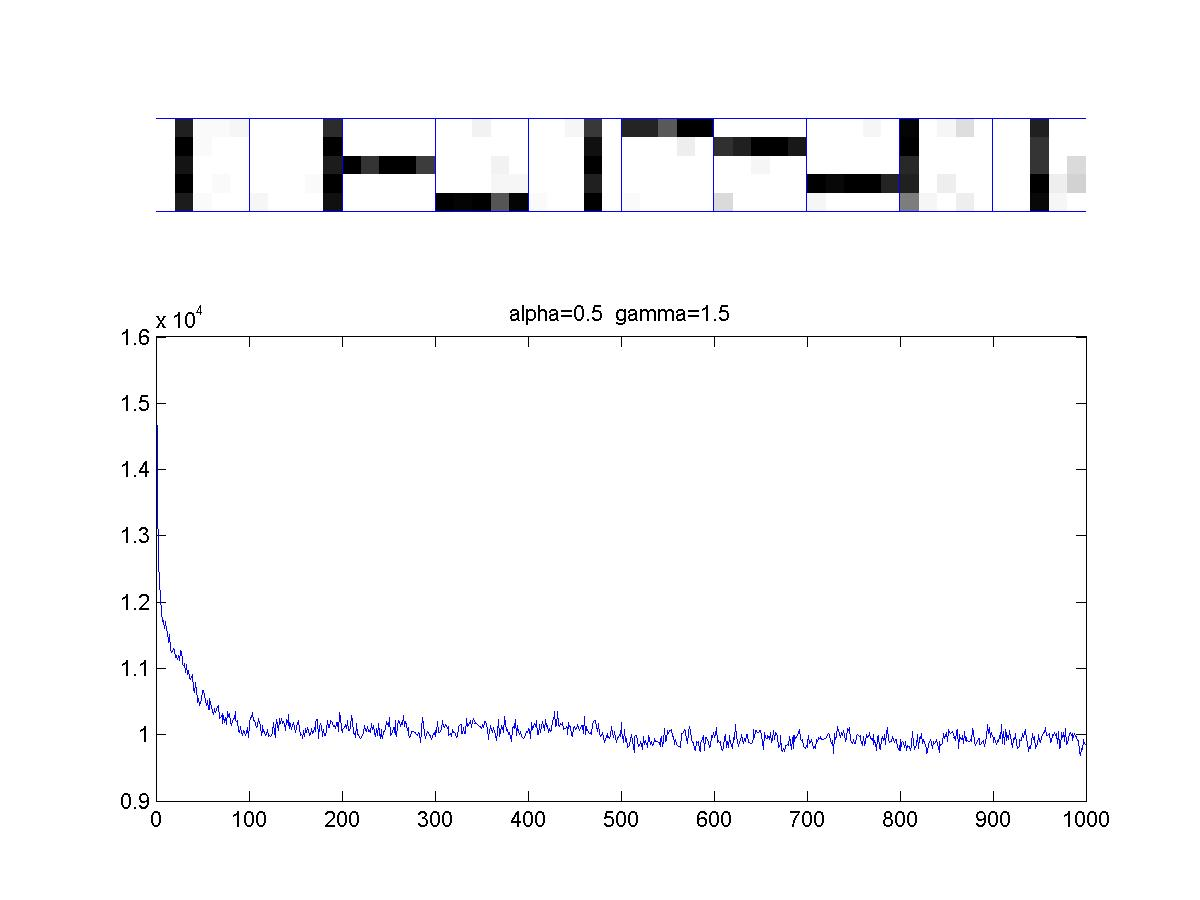
\includegraphics[width=3in,height=2in]{exp_gib.jpg} 
    \caption{Gibbs}
    \label{fig:by:table}  
   \end{minipage}% 
\end{figure}

\begin{figure}[h] 
  \begin{minipage}[b]{0.5\textwidth} 
    \centering 
    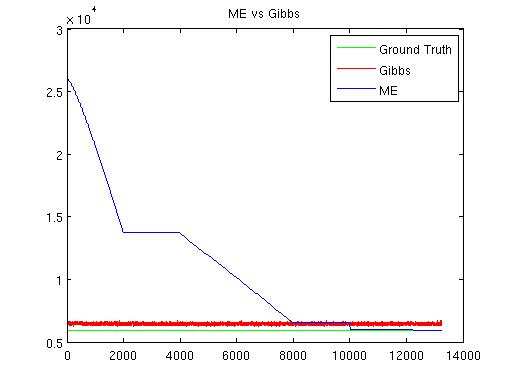
\includegraphics[width=3in,height=2in]{hdp_com.jpg} 
    \caption{ME vs Gibbs} 
    \label{fig:by:table} 
  \end{minipage}% 
  \begin{minipage}[b]{0.5\textwidth} 
    \centering 
    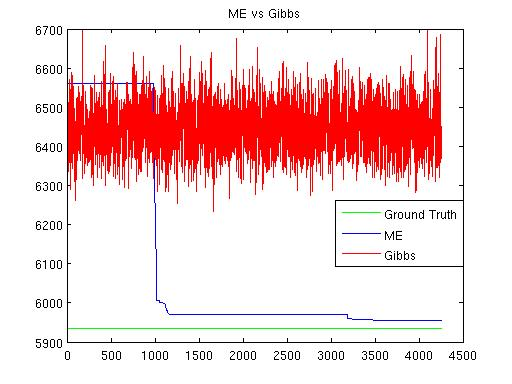
\includegraphics[width=3in,height=2in]{hdp_com2.jpg} 
    \caption{ME vs Gibbs}
    \label{fig:by:table}  
   \end{minipage}% 
\end{figure}

\section{1) Formula}
W:number of unique words\\ 
$n_{..k}^{w}$number of occurence of word w in dish k \\ \\
$-log p(x|z,\lambda)$\\ =\\
(Likelihood-term)$ \sum_{k=1}^{K} [log(\frac{\Gamma(n_{..k}+W\phi_{0})}{\Gamma(W\phi_{0})})+\sum_{w=1}^{W}log(\frac{\Gamma(\phi_{0})}{\Gamma(\phi_{0}+n_{..k}^{w})})]$
\\
+
\\
(Allocation-term)$\underline{\sum_{j=1}^{J}\{log \frac{\Gamma(n_{j..}+\alpha)}{\Gamma(\alpha)}-\sum_{t=1}^{m_{j.}}[log(\Gamma(n_{jt.})+log \alpha]\}+
 log \frac{\Gamma(T+\gamma)}{\Gamma(\gamma)}-\sum_{k=1}^{K} [log(\Gamma(m_{.k})+log \gamma]}$
\\ \\ \\
=\\
(t-term)$ \underline{log \frac{\Gamma(T+\gamma)}{\Gamma(\gamma)}+\sum_{j=1}^{J} \{log \frac{\Gamma(n_{j..}+\alpha)}{\Gamma(\alpha)}-\sum_{t=1}^{m_{j.}}[log(\Gamma(n_{jt.})+log \alpha
]\}}$\\ \\
+(k-term)$ \sum_{k=1}^{K} [log(\frac{\Gamma(n_{..k}+W\phi_{0})}{\Gamma(W\phi_{0})})+log(\Pi_{w=1}^{W}\frac{\Gamma(\phi_{0})}{\Gamma(\phi_{0}+n_{..k}^{w})})
-\underline{log(\Gamma(m_{.k})-log \gamma]}$\\ \\ 


\section{2) Initialization?}

\subsection{i)Extreme Case}
Bottom-up Initialization: All customers are assigned to different tables with different dishes.\\
Top-down Initialization: Every Restaurant has only one table with the same dish.\\ \\
We know they are of no good since they don't capture potential mixture components.\\ \\
Indicated by the toy bar example, with these initialization, ME algorithm quickly get stuck at the configuration: 1 table for each restaurant,
where the t-term$\sim$ 200,k-term$\sim$ 6,000 while for the ground truth:t-term$\sim$ 3,000,k-term$\sim$ 3,000
\subsection{ii)Somewhere in Between}
Hoping that some restaurant may have only one mixture component,we have the following initializaiton:\\ \\
For each of the J restaurants independently:\\
\begin{enumerate}
 
\item Make J-1 tables serving J-1 dishes, where each dish is informed by all the data from one of the other restaurants
\item  Search over assignments $t_{ji}$ of customers to these tables (keep $k_{jt}$ fixed and don't allow the option of making a new table$\&$dish not shared with any other restaurant)
\item  Store the at most J-1 tables with at least one customer (hopefully this will be a number bigger than one but much less than J-1)

\end{enumerate}

But the problems are:\\ 
\begin{enumerate}
\item {\bf It may be equivalent to simply assigning customers with the same type(word) to the same table.} \\
Suppose we have 40 Restaurants, each has 50 customers.\\
For the 50 customers in Restaurant 1, they have 39 tables(each formed by a restaurant) to choose from.\\
For the first customer(say with word $w_{0}$), t-term is the same for assigning it any of the 39 tables(since $n_{jt}$=50 for all in this case)\\
The difference among the k-term happens at$log\frac{1}{\Gamma(\phi_{0}+n_{..k}^{w_{0}})}$ which is concave(bigger $n_{..k}^{w_{0}}$,bigger decrease)\\
Thus assign the first customer to the table with the highest count of word $w_{0}$ will mostly decrease the Free Energy(Negative log Probability).
\item  In the toy bar data, unfortunately, the highest count of a certain word happens at the cross of two bars in a restaurant, which still does not capture
any correlation among the word. As a result, in every restaurant, each different type of word is assigned to a different table, which doesnot 
incorporate any potential topic information.
\item {\bf Tricks:} For the toy bar data, we know the ture mixture components and actually we can roughly recover them by {\bf finer} pre-processing the tables 
instead of roughly making them out of each restaurant.
\end{enumerate}

\subsection{iii)Experiment}
1)I tried the new Initialization, which forces dishes to have only single word.\\
2)I tried to initialize with the result from Gibbs Sampling, which works well.\\
{\bf(The "Ground Truth" is made up...since there are exponentially many 
configurations even though we know the true mixture components)}\\
\begin{figure}[h] 
  \begin{minipage}[b]{0.5\textwidth} 
    \centering 
    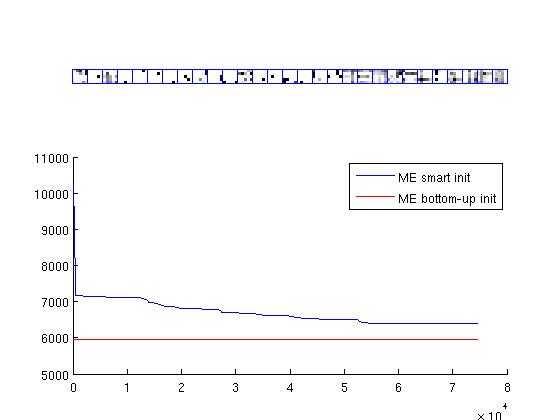
\includegraphics[width=3in,height=2in]{new_init.jpg} 
    \caption{somewhere in between initializaiton} 
    \label{fig:by:table} 
  \end{minipage}% 
  \begin{minipage}[b]{0.5\textwidth} 
    \centering 
    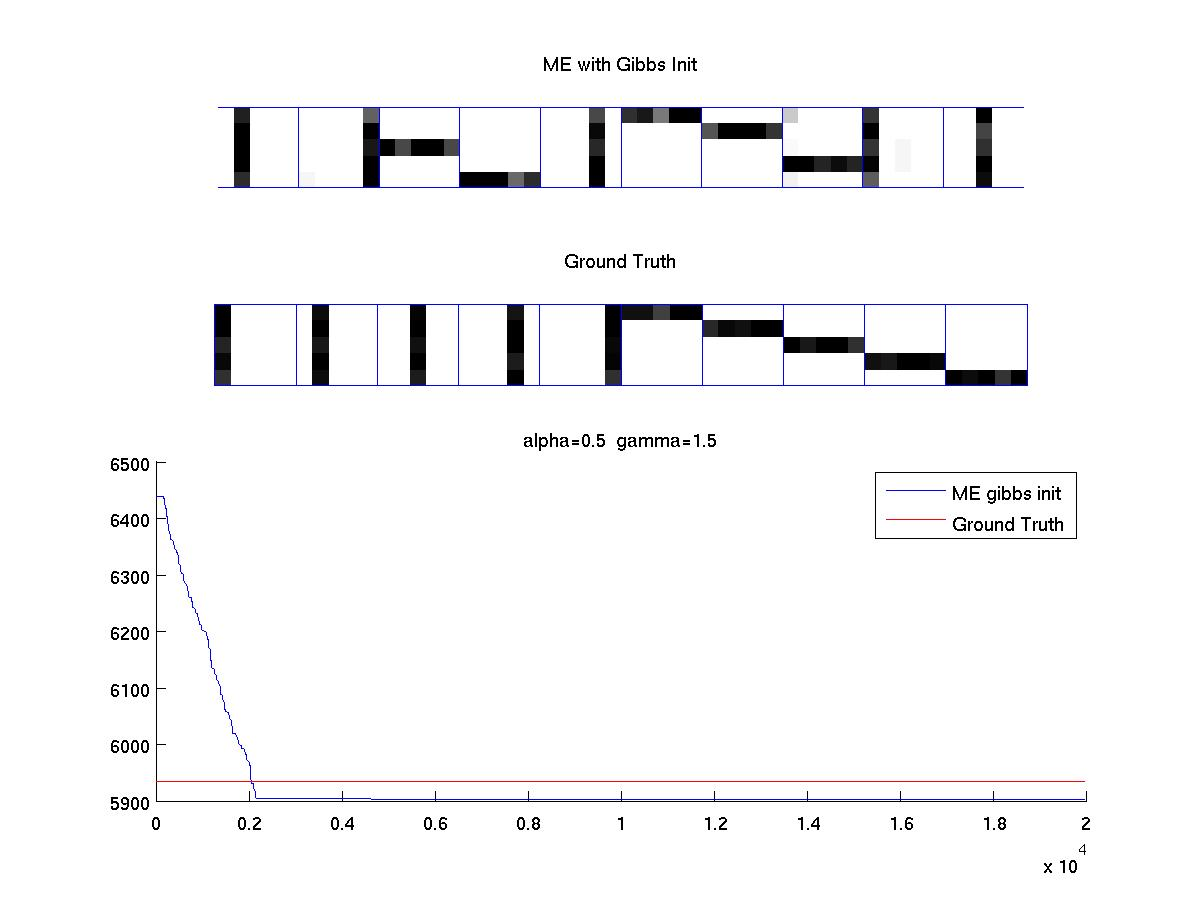
\includegraphics[width=3in,height=2in]{gibbs_init.jpg} 
    \caption{Gibbs Initialization}
    \label{fig:by:table}  
   \end{minipage}% 
\end{figure}

\section{3) Searching Scheme?}
{\bf What do we really want?}(log probability is definitely not the answer)\\ \\ \\
Take the toy bar data as an example.\\
Given 25 words,40 Restaurants each of which is a mixture of bars.\\ \\
{\bf Clue1:   Each dish has its own vocabulary,one of $2^{25}-1$ nonempty subsets of (1,...,25). 
We want these dishes to be the true mixture component(bars) to construct each restaurant}\\ \\
{\bf Clue2:   In the object function, most terms can be organized into "partition cost".e.g.$\frac{\Gamma(n_{..k}+W\phi_{0})}{\Pi_{1}^{W}\Gamma(\phi_{0}+n_{..k}^{w})}$
 is the cost to divide dish vocabulary into each word. The bigger the partition component, the smaller the cost}\\ \\



Want to minimize:$-log p(x|z,\lambda)$\\ =\\
(Smaller Dish vocabulary term)$ log[\Pi_{k=1}^{K}(\frac{\Gamma(n_{..k}+W\phi_{0})}{\Pi_{1}^{W}\Gamma(\phi_{0}+n_{..k}^{w})})]-Tlog\alpha-Klog\gamma$\\ 
(Bigger Dish vocabulary term)$+Klog\frac{\Gamma(\phi_{0})^{W}}{\Gamma(W\phi_{0})}+log\frac{\Gamma(T+\gamma)}{\Pi_{k=1}^{K}\Gamma(m_{.k})}+log \Pi_{j=1}^{J}\frac{\Gamma(n_{j..})}{\Pi_{t=1}^{m_{j}}\Gamma(n_{jt.})}$\\
(constant-term)$-log\Gamma(\gamma)-Jlog(\Gamma(\alpha))+log \Pi_{j=1}^{J}\frac{\Gamma(n_{j..}+\alpha)}{\Gamma(n_{j..})}$
\\ \\
Fixing $\alpha,\gamma$:\\
\begin{enumerate}
\item Smaller Dish vocabulary term:
\begin{enumerate}[(a)]
\item $\frac{\Gamma(n_{..k}+W\phi_{0})}{\Pi_{1}^{W}\Gamma(\phi_{0}+n_{..k}^{w})}$ wants the dish to have bigger partition component (concentrated on some of the words).\\
e.g. $\frac{\Gamma(10)}{\Gamma(5)\Gamma(5)}<<\frac{\Gamma(10)}{\Gamma(1)...\Gamma(1)}$
\item Consequently, smaller dish vocabulary may need more dishes K and more tables T to explain each Restaurant:$-Tlog\alpha-Klog\gamma$
\end{enumerate} 
\item Bigger dish vocabulary term:
\begin{enumerate}[(a)]
\item $log \Pi_{j=1}^{J}\frac{\Gamma(n_{j..})}{\Pi_{t=1}^{m_{j}}\Gamma(n_{jt.})}$ wants each restaurant has only one table, thus a big dish vocabulary.
\item $log\frac{\Gamma(T+\gamma)}{\Pi_{k=1}^{K}\Gamma(m_{.k})}$ wants smaller number of dishes:\\
e.g. $\frac{\Gamma(10)}{\Gamma(5)\Gamma(5)}<<\frac{\Gamma(10)}{\Gamma(1)...\Gamma(1)}$

\item Consequently, bigger dish vocabulary may need less dishes K to explain each Restaurant:$Klog\frac{\Gamma(\phi_{0})^{W}}{\Gamma(W\phi_{0})}$

\end{enumerate} 
\end{enumerate} 
\end{spacing}
\end{document}

%%%%%%%%%%%%%%%%%%%%%%%%%%%%%%%%%%%%%%%%%%%%%%%%%%%%%%%%%%%%%
